\chapter{Floating and Sinking}\label{ch:g1:floating-and-sinking}

Drop a pebble in a puddle: it disappears to the bottom. Drop a leaf:
it rides on top like a little boat. Bath time, puddles and ponds all
ask the same question --- what \omterm{def:g1:floating-and-sinking:words}{floats}, what \omterm{def:g1:floating-and-sinking:words}{sinks}, and can we guess
before we drop it in?

\section{Float or sink?}

\begin{definition}[Floating and sinking]\label{def:g1:floating-and-sinking:words}
A thing \emph{floats}\index{float} when the water holds it up at the
top; it \emph{sinks}\index{sink} when it goes down to the bottom.
A cork floats; a pebble sinks.
\end{definition}

\begin{method}[A fair float test]\label{met:g1:floating-and-sinking:test}
\begin{enumerate}
  \item Fill a big bowl (or the sink) with water;
  \item put the object on the water \emph{gently} --- no throwing:
        a splash can push even a floater under for a moment;
  \item let go completely, and wait while you count to $5$;
  \item look: on top is a floater, at the bottom is a sinker.
\end{enumerate}
Test each object the same way, so the comparison is fair.
\end{method}

\begin{example}[Try it: the sorting game]\label{ex:g1:floating-and-sinking:sorting}
Gather a cork, a coin, a plastic spoon, a metal spoon, a pebble, a
pencil and a dry leaf, and test them one by one with
\cref{met:g1:floating-and-sinking:test}. Floaters: the cork, the
plastic spoon, the pencil, the leaf. Sinkers: the coin, the metal
spoon, the pebble. Before each drop, say your guess out loud ---
that is what scientists call a \emph{prediction}, and being wrong is
half the fun.
\end{example}

\begin{omfigure}
\begin{tikzpicture}[scale=0.85]
  \draw[thick] (0,0) -- (0,3.2) (0,0) -- (9,0) (9,0) -- (9,3.2);
  \fill[omDef, opacity=0.15] (0,0) rectangle (9,2.6);
  % cork: a little cylinder riding half-sunk
  \draw[thick, fill=brown!45] (1.25,2.38) rectangle (1.75,2.78);
  \draw[thick, fill=brown!30] (1.5,2.78) ellipse (0.25 and 0.08);
  \node[above, font=\small] at (1.5,3.0) {cork};
  % leaf: pointed oval with a midrib, flat on the surface
  \draw[thick, green!45!black, fill=green!40]
    (3.6,2.62) .. controls (4.0,2.92) and (4.5,2.92) .. (4.85,2.62)
    .. controls (4.5,2.52) and (4.0,2.52) .. (3.6,2.62);
  \draw[green!45!black] (3.68,2.63) -- (4.78,2.63);
  \draw[thick, green!45!black] (3.6,2.62) -- (3.42,2.56);
  \node[above, font=\small] at (4.2,3.0) {leaf};
  % pencil: yellow body, sharpened tip, lying on the water
  \draw[thick, fill=red!45] (5.95,2.56) rectangle (6.1,2.76);
  \draw[thick, fill=yellow!75] (6.1,2.56) rectangle (7.6,2.76);
  \draw[thick, fill=brown!35] (7.6,2.56) -- (7.95,2.66)
    -- (7.6,2.76) -- cycle;
  \fill[black] (7.95,2.66) -- (7.85,2.62) -- (7.85,2.7) -- cycle;
  \node[above, font=\small] at (6.9,3.0) {pencil};
  % pebble: an irregular gray lump on the bottom
  \draw[thick, fill=omExo!55]
    (2.25,0.18) .. controls (2.3,0.45) and (2.75,0.52) .. (2.95,0.32)
    .. controls (3.05,0.18) and (2.9,0.04) .. (2.6,0.04)
    .. controls (2.4,0.04) and (2.25,0.06) .. (2.25,0.18);
  \node[above, font=\small] at (2.6,0.6) {pebble};
  % coin: a flat golden disc
  \draw[thick, fill=yellow!70!orange] (5.15,0.04) rectangle (5.65,0.12);
  \draw[thick, fill=yellow!85!orange] (5.4,0.12) ellipse (0.25 and 0.07);
  \node[above, font=\small] at (5.4,0.45) {coin};
  % metal spoon: bowl plus handle
  \draw[thick, fill=omExo!40] (7.05,0.2) ellipse (0.34 and 0.16);
  \draw[line width=2.4pt, omExo!80!black] (7.38,0.16) -- (8.5,0.08);
  \node[above, font=\small] at (7.8,0.55) {metal spoon};
  % the water in front of everything, and its surface line
  \fill[omDef, opacity=0.12] (0,0) rectangle (9,2.6);
  \draw[omDef, thick] (0,2.6) -- (9,2.6);
\end{tikzpicture}

{\small After the sorting game: floaters ride the top of the water,
sinkers rest on the bottom.}
\end{omfigure}

\begin{omfigure}
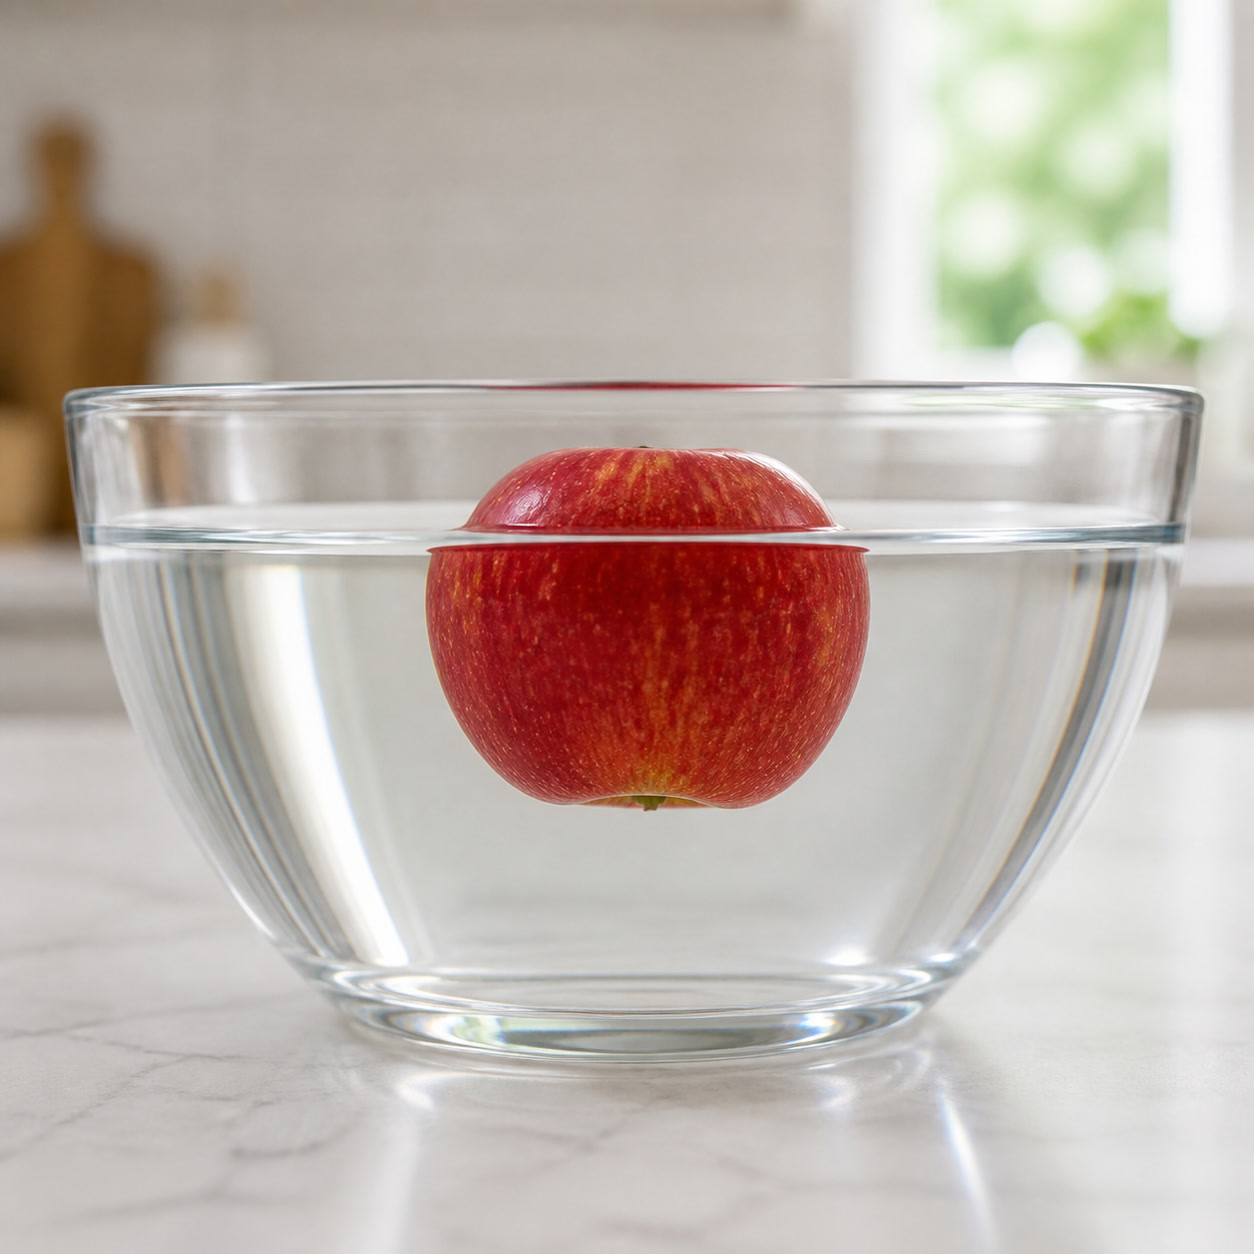
\includegraphics[width=0.42\linewidth]{images/book1/ai/g1-floating-apple.jpg}

{\small An apple floating in a bowl of water: it rides low, most of its body under the surface --- yet it \omterm{def:g1:floating-and-sinking:words}{floats}.}
\end{omfigure}

\section{Heavy is not the whole story}

Many people guess ``heavy things \omterm{def:g1:floating-and-sinking:words}{sink}, \omterm{def:g1:light-and-shadows:source}{light} things \omterm{def:g1:floating-and-sinking:words}{float}''. The
water has a surprise for them.

\begin{example}[The log and the coin]\label{ex:g1:floating-and-sinking:log}
A fallen tree trunk is far too heavy for you to lift --- yet it
\omterm{def:g1:floating-and-sinking:words}{floats} down the river. A little coin weighs less than a cookie ---
yet it \omterm{def:g1:floating-and-sinking:words}{sinks} straight away. So heavy-or-light cannot be the whole
rule: the huge log \omterm{def:g1:floating-and-sinking:words}{floats} while the tiny coin drowns.
\end{example}

\begin{example}[It is the stuff that counts]\label{ex:g1:floating-and-sinking:stuff}
Look back at the sorting game: the plastic spoon floated and the
metal spoon sank, though they have the same shape and the same job.
What made the difference is the \emph{stuff} they are made of ---
wood and cork and most plastics are floating stuffs; metal, stone and
glass are sinking stuffs. A thing usually behaves like its stuff:
wood \omterm{def:g1:floating-and-sinking:words}{floats} whether it is a twig or a whole trunk.
\end{example}

\begin{remark}[A pinch of mystery]\label{rem:g1:floating-and-sinking:why}
\emph{Why} does wood \omterm{def:g1:floating-and-sinking:words}{float} and metal \omterm{def:g1:floating-and-sinking:words}{sink}? That is a real question,
and its full answer is one of the treasures of this course --- it
needs ideas that arrive in later years. For now we collect good
observations; the ``why'' will find us ready.
\end{remark}

\section{The water pushes back}

\begin{example}[Try it: push the ball under]\label{ex:g1:floating-and-sinking:push}
Take a floating ball in the bath and push it slowly underwater with
your palm. Feel that? The water pushes it back up, harder the deeper
you push --- and if your hand slips, the ball leaps out of the water.
The water is not just \emph{letting} floaters sit on top: it is
actively holding them up, like your hands holding a baby.
\end{example}

\begin{omfigure}
\begin{tikzpicture}[scale=0.85]
  \draw[thick] (0,0) -- (0,3.4) (0,0) -- (6.5,0) (6.5,0) -- (6.5,3.4);
  \draw[omDef, thick] (0,2.7) -- (6.5,2.7);
  \fill[omDef, opacity=0.15] (0,0) rectangle (6.5,2.7);
  \draw[thick, fill=white] (3.2,1.5) circle (0.6);
  \node[font=\small] at (3.2,1.5) {ball};
  \draw[-Stealth, very thick, omThm] (3.2,3.3) -- (3.2,2.25);
  \node[right, font=\small, omThm] at (3.35,2.9) {your hand pushes down};
  \draw[-Stealth, very thick, omDef] (3.2,0.35) -- (3.2,0.85);
  \node[right, font=\small, omDef] at (3.35,0.55) {the water pushes up};
\end{tikzpicture}

{\small A ball held underwater: your hand pushes down, the water
pushes up. Let go, and the water's push wins.}
\end{omfigure}

\begin{example}[The plasticine boat]\label{ex:g1:floating-and-sinking:boat}
Roll a lump of plasticine into a ball and drop it in the water: it
\omterm{def:g1:floating-and-sinking:words}{sinks} --- plasticine is a sinking stuff. Now take the \emph{same}
lump and shape it into a little bowl with high sides, and set it
gently on the water: it \omterm{def:g1:floating-and-sinking:words}{floats}! Same stuff, same lump --- only the
shape changed. A wide, hollow shape gives the water more to push up
on. That is the secret of the great ships: metal is a sinking stuff,
but a metal hull is shaped like a huge hollow bowl.
\end{example}

\begin{omfigure}
\begin{tikzpicture}[scale=0.85]
  \draw[thick] (0,0) -- (0,2.6) (0,0) -- (4.6,0) (4.6,0) -- (4.6,2.6);
  \draw[omDef, thick] (0,2.0) -- (4.6,2.0);
  \fill[omDef, opacity=0.15] (0,0) rectangle (4.6,2.0);
  \fill[omThm] (2.3,0.35) circle (0.35);
  \node[below, font=\small] at (2.3,-0.2) {plasticine ball: sinks};
  \draw[thick] (6.4,0) -- (6.4,2.6) (6.4,0) -- (11,0)
    (11,0) -- (11,2.6);
  \draw[omDef, thick] (6.4,2.0) -- (11,2.0);
  \fill[omDef, opacity=0.15] (6.4,0) rectangle (11,2.0);
  \draw[thick, omThm, fill=white]
    (7.9,2.25) -- (8.1,1.75) -- (9.3,1.75) -- (9.5,2.25);
  \node[below, font=\small] at (8.7,-0.2) {same lump as a bowl: floats};
\end{tikzpicture}

{\small One lump of plasticine, two shapes, two fates. The hollow
bowl shape gives the water more to hold up.}
\end{omfigure}

\section{Exercises}

\begin{exercise}[$\star$]\label{exo:g1:floating-and-sinking:1}
Sort into floaters and sinkers: a cork; \ a key; \ a dry twig; \ a
marble; \ a plastic duck; \ a stone.
\end{exercise}

\begin{exercise}[$\star$]\label{exo:g1:floating-and-sinking:2}
In \cref{met:g1:floating-and-sinking:test}, why must you put the
object on the water gently instead of throwing it in?
\end{exercise}

\begin{exercise}[$\star$]\label{exo:g1:floating-and-sinking:3}
Before testing, Nora guesses: ``The metal spoon will \omterm{def:g1:floating-and-sinking:words}{float} because
spoons \omterm{def:g1:floating-and-sinking:words}{float}.'' What happened in the sorting game? What should Nora
look at instead of the shape's job: the stuff or the name?
\end{exercise}

\begin{exercise}[$\star$]\label{exo:g1:floating-and-sinking:4}
Give one thing that is heavy and \omterm{def:g1:floating-and-sinking:words}{floats}, and one thing that is \omterm{def:g1:light-and-shadows:source}{light}
and \omterm{def:g1:floating-and-sinking:words}{sinks}. What does this show about the guess ``heavy things
\omterm{def:g1:floating-and-sinking:words}{sink}''?
\end{exercise}

\begin{exercise}[$\star$]\label{exo:g1:floating-and-sinking:5}
A twig \omterm{def:g1:floating-and-sinking:words}{floats}. Will a whole tree trunk \omterm{def:g1:floating-and-sinking:words}{float} too? Which example of
the chapter helps you answer?
\end{exercise}

\begin{exercise}[$\star$]\label{exo:g1:floating-and-sinking:6}
Push a floating ball underwater in the bath and let go. What do you
feel while pushing, and what does the ball do when you let go?
\end{exercise}

\begin{exercise}[$\star$]\label{exo:g1:floating-and-sinking:7}
Ships are made of metal, and metal is a sinking stuff. What shape
saves the ship? Which experiment of the chapter shows it?
\end{exercise}

\begin{exercise}[$\star$]\label{exo:g1:floating-and-sinking:8}
Test at bath time: does a full, closed bottle of water \omterm{def:g1:floating-and-sinking:words}{float} or
\omterm{def:g1:floating-and-sinking:words}{sink}? And the same bottle empty, with its cap on? Say your guesses
first, then try.
\end{exercise}

\begin{exercise}[$\star\star$]\label{exo:g1:floating-and-sinking:9}
Leo's plasticine boat \omterm{def:g1:floating-and-sinking:words}{floats} nicely --- until he squashes it back
into a ball, and it \omterm{def:g1:floating-and-sinking:words}{sinks}. ``The water got tired of holding it,''
says Leo. Give a better explanation, using
\cref{ex:g1:floating-and-sinking:boat}.
\end{exercise}
